\documentclass[main.tex]{subfiles}

\begin{document}

\counterwithout{equation}{subsection}

\section*{Анализ трещины гидроразрыва пласта постоянной высоты (Е.В. Донцов, 26 октября 2021)}
\addcontentsline{toc}{section}{Анализ трещины гидроразрыва пласта постоянной высоты (Е.В. Донцов)}

\textbf{Аннотация}

В данной работе проводится анализ задачи о трещине гидроразрыва пласта постоянной высоты.
Предполагается, что трещина распространяется при закачке ньютоновской жидкости, и в модель также включены эффекты трещиностойкости и утечки.
В первую очередь представлен анализ области кончика для такой трещины.
Исследуются предельные решения и их расположение в двумерном параметрическом пространстве.
Кроме того, строится приближенное решение задачи и проверяется его точность во всем параметрическом пространстве.
Затем представлен анализ конечной трещины.
Получены аналитические выражения для предельных решений.
Построено полное численное решение, а также разработана аппроксимация, основанная на решении для области кончика и на глобальном балансе объемов.
Численное решение используется для проверки точности аппроксимации, а сама аппроксимация используется для исследования всего параметрического пространства задачи.
Это, в свою очередь, позволяет определить зоны применимости предельных решений, которые в дальнейшем можно использовать для количественной оценки того, какие параметры задачи наиболее сильно влияют на динамику трещины.

\subsection{Введение}

Трещины ГРП чаще всего создаются под землей с целью повышения нефтеотдачи и газоотдачи пластов [1].
В настоящее время для моделирования такого явления без особого труда используются сложные численные модели, которые могут учитывать распространение одной или нескольких трещин ГРП, взаимодействие между трещинами, перенос проппанта, тепловые эффекты, химические эффекты, эффекты многофазного потока и т. д.
Тем не менее, понимания основных механизмов и поведения трещин гидроразрыва лучше достигать с помощью простых моделей, которые фокусируются на конкретном аспекте проблемы, игнорируя при этом остальные сложности.
Это относится к данному исследованию относительно простой геометрии трещины гидроразрыва пласта постоянной высоты.

Существует множество <<простых>> моделей трещины гидроразрыва пласта.
Слово <<простой>> здесь по существу означает, что математическая формулировка задачи является одномерной.
В результате такого математического упрощения можно более детально исследовать задачу и лучше понять структуру решения.
Первый пример — задача о полубесконечной трещине гидроразрыва, являющаяся моделью кончика конечной планарной трещины [2, 3, 4].
Предельные аналитические решения задачи были впервые получены в [5] и [6] для случая доминирования вязкости и утечек соответственно.
Последнее предельное решение, соответствующее доминированию трещиностойкости, вытекает из классической Механики Линейно-Упругого Разрушения (LEFM) [7].
Общее решение задачи, учитывающее ньютоновскую жидкость, Картерову утечку и трещиностойкость, получено в [3].
Позднее в [8] было получено быстрое приближение для этого решения, которое затем было использовано в качестве условия распространения в планарной модели трещины гидроразрыва [9].
Также стоит упомянуть многочисленные расширения модели, которые учитывают степенные жидкости [10], жидкости Гершеля-Балкли [11], жидкости Карро [12], эффект отставания жидкости [13], эффект турбулентного течения [14], эффект когезионной зоны [15], эффект проппанта [16] и эффект утечки, зависящей от давления [17].
Эта модель уже показывает, как можно понять множественные физические эффекты, рассматривая относительно простой сценарий.

Трещины в условиях плоской деформации и радиальные трещины гидроразрыва можно считать <<простыми>> геометриями, поскольку математическая формулировка для них также является одномерной.
В отличие от полубесконечной трещины, для которой существует три предельных решения, конечная трещина имеет четыре предельных случая.
Обратите внимание, что это относится только к модели, в которой учитываются эффекты трещиностойкости, вязкости и утечек Картера, т.е. игнорируются эффекты запаздывания жидкости, когезионной зоны, сложной реологии жидкости и т.д.
Вышеупомянутые четыре случая определяются конкуренцией между трещиностойкостью трещины и вязкостью флюида, а также запасом флюида внутри трещины или внутри горной формации.
Поэтому эти пределы определяются следующим образом: Storage-Toughness (доминирование трещиностойкости при малых утечках), Storage-Viscosity (доминирование вязкости при малых утечках), Leak-off-Toughness (доминирование трещиностойкости при больших утечках) и Leak-off-Viscosity (доминирование вязкости при больших утечках), см. к примеру обзорную статью [18].
Ранние исследования были сосредоточены преимущественно на поиске решений для этих предельных случаев [19, 20, 21, 22].
Первый анализ полной задачи дан в [23] для случая трещины в условиях плоской деформации и в [24] для случая радиальной геометрии.
Альтернативный анализ для этих задач был представлен в [25, 26].
Быстрое приближенное решение глобальной задачи строится с использованием полубесконечного решения (или решения для кончика трещины) [8] и глобального баланса объема.
Такое быстрое решение позволило просканировать всё параметрическое пространство и построить карту решений, определяющую области применимости предельных решений.
Позже аналогичная концепция использовалась для анализа влияния анизотропии и степенной реологии на параметрическое пространство в [27], для исследования влияния когезионной зоны в [15] и для построения сверхбыстрого симулятора ГРП в [28].

Последней, но не менее важной, <<простой>> геометрией является трещина гидроразрыва постоянной высоты или трещина Перкинса-Керна-Нордгрена (PKN) [29, 30].
Технически в список <<простых>> случаев можно включить и псевдотрехмерную модель [31, 32, 33].
Но она заметно сложнее в том смысле, что её параметрическое пространство больше (шире), что делает анализ более сложным.
Классическая модель PKN не учитывает влияние трещиностойкости, а учитывает только вязкость и утечку.
Решения с преобладанием вязкости и утечек можно найти в [1].
Анализ области кончика, опять же при отсутствии трещиностойкости, выполнен в [34].
Лабораторные наблюдения, подтверждающие предсказанное поведение вблизи кончика, подытожены в [35].
Отметим, что для этой геометрии трещины также проводится анализ эффектов турбулентного течения [36, 37].
Во всех приведенных выше исследованиях не рассматривается влияние трещиностойкости на решение.
Есть два подхода включения трещиностойкости в модель.
Первый подход был предложен в [38], в нём граничное условие на давление на кончике берётся из условия для радиальной трещины с однородным давлением.
Позднее это условие было пересмотрено в [39], где авторы предложили несколько изменить его, исходя из энергетических соображений.
Второй подход заключается в замене соотношения локальной упругости, используемого в классической модели PKN, более точным нелокальным выражением, которое можно комбинировать со стандартным критерием распространения LEFM [40].
Хотя показано, что второй подход более точен [40], с его помощью сложнее проводить анализ.
Поэтому в данном исследовании используется модель с локальной упругостью и граничным условием конечного давления на кончике трещины.

Как видно из приведенного выше обзора литературы, параметрические пространства для всех <<простых>> моделей, кроме случая PKN, были тщательно проанализированы для случая, когда модель учитывает одновременное взаимодействие между трещиностойкостью, вязкостью и утечкой.
Вероятно, это связано с тем, что процедура учета влияния трещиностойкости в модели PKN была введена сравнительно недавно.
Чтобы заполнить пробел, эта работа направлена на исследование параметрического пространства для области кончика трещины PKN, т.е. расширение работы [34] на случай влияния трещиностойкости.
Кроме того, более крупной задачей данной работы является тщательное исследование параметрического пространства для конечной трещины и определение всех предельных решений и зон их применимости в параметрическом пространстве.
В частности, структура данной работы такова.
Раздел 2 описывает основные уравнения для рассматриваемой задачи.
Затем в разделе 3 анализируется задача о концевой области и строится параметрическая карта для этой задачи.
После этого в разделе 4 представлены вершинные решения для конечной трещины PKN.
Параметрическая карта для конечной трещины построена в разделе 5 с использованием быстрого приближенного решения, которое сравнивается с более точным численным решением.
Наконец, в разделе 6 представлены примеры применения, а в разделе 7 подведены итоги.


\subsection{Основные уравнения}

Рассмотрим задачу о трещине гидроразрыва постоянной высоты или просто трещине PKN, изображенной на рис. 1(а).
Пусть трещина вертикальна и занимает плоскость $(x, y)$, причем $y$— вертикальная координата, а $x$ — горизонтальная координата.
Пусть $H$ — высота трещины, $l$ — полудлина.
Высота $H$ считается постоянной для всей трещины, а длина является функцией времени.
Также предполагается, что $H\ll l$, что позволяет упростить основные уравнения до одномерных.

\begin{figure}[H]
\center
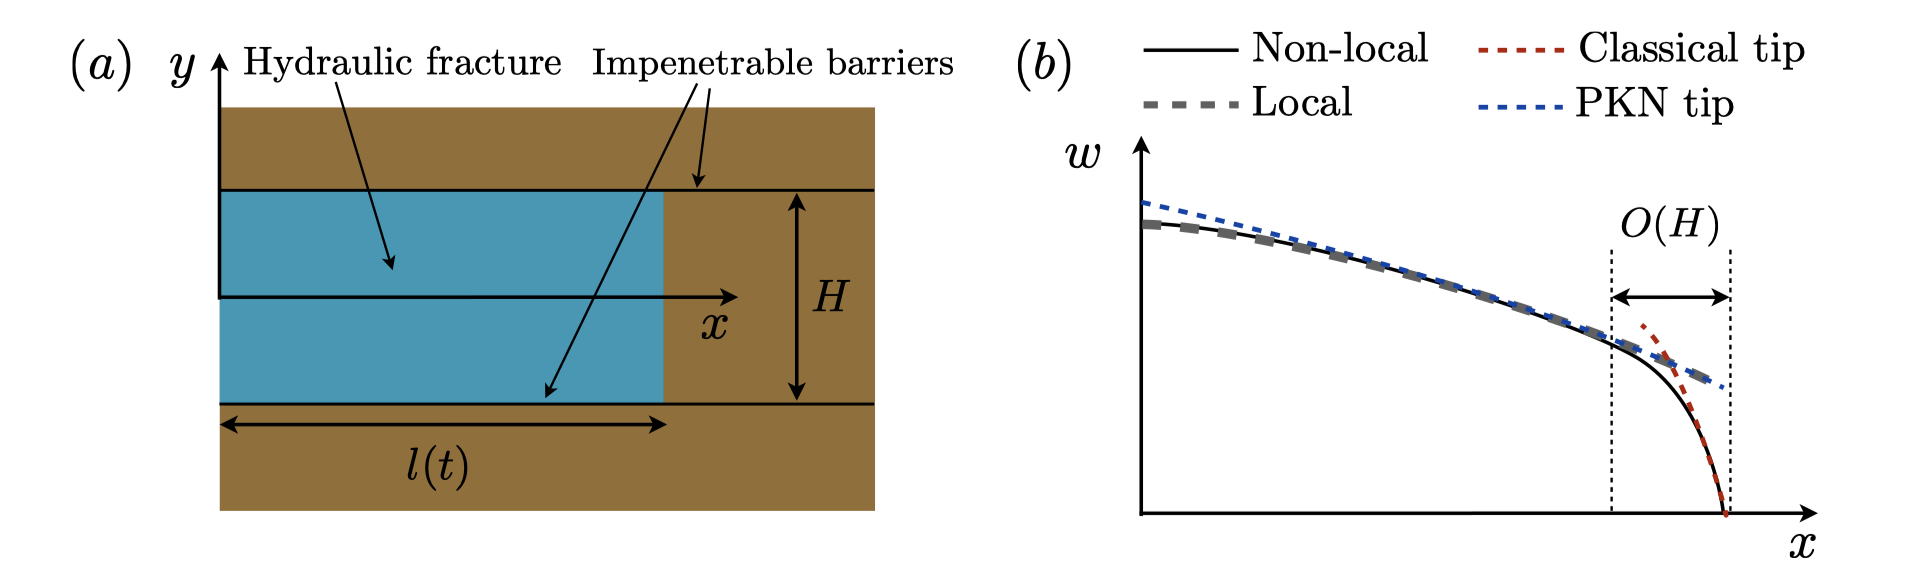
\includegraphics[width=\textwidth]{Dontsov-2021-fig1}
\vspace*{-10mm}
\caption{(a) Схема трещины гидроразрыва постоянной высоты. (b) Зависимость ширины трещины $w$ от координаты $x$ для разных моделей}
\label{fig:Dontsov-2021-fig1}
\end{figure}

Различные решения задачи и их асимптоты схематично показаны на рис.1(б).
Черная линия указывает на наиболее точное решение, использующее соотношение нелокальной упругости.
Она имеет классическую концевую асимптотику, вытекающую из задачи о полубесконечной трещине с плоской деформацией (штриховая красная линия).
Пунктирная серая линия указывает на решение, в котором используется локальная упругость вместе с граничным условием давления на конце, чтобы уловить эффект трещиностойкости.
Это приводит к прерывистому поведению ширины трещины на кончике.
Хотя это граничное условие и не является физическим, оно на самом деле означает поведение на некотором расстоянии от кончика $O(H)$.
Действительно, как показано в [40], решения с локальной и нелокальной упругостью сближаются друг с другом при удалении от кончика трещины, а различия сосредоточены в области $O(H)$ вблизи кончика.
Общие характеристики трещины, такие как длина и ширина в стволе скважины, фиксируются точно, так как $H\ll l$.
Кроме того, можно также рассмотреть асимптотику кончика для трещины PKN, которая схематично показана пунктирной синей линией.
Она справедлива на расстояниях, соизмеримых с длиной трещины l, в отличие от классической асимптоты (штриховая красная линия), которая точна на расстояниях порядка высоты трещины $H$ для рассматриваемой геометрии.
Для упрощения анализа в данном исследовании рассматривается модель с локальной эластичностью.

Используя классические допущения модели PKN [29, 30], каждое поперечное сечение вертикальной трещины считается эллиптическим, а давление определяется на основе допущения выполнения условия локальной плоской деформации.
Это означает, что
\beq
w(x,y)=\frac{4}{\pi}\bar{w}(x)\sqrt{1-\left(\frac{2y}{H}\right)^2};\,\,\,\,\,
p(x)=\frac{2E'\bar{w}(x)}{\pi H};\,\,\,\,\,
\bar{w}(x)=\frac{1}{H}\int\limits_{-H/2}^{H/2}{w(x,y)dy},
\eeq
где $w(x,y)$ -- раскрытие трещины,
$\bar{w}(x)$ -- эффективная ширина,
$p(x)$ -- давление жидкости,
$E'=E/(1-\nu^2)$ -- модуль Юнга плоской деформации.
В предположении $H\ll l$, усреднённые по вертикали уравнения для случая ньютоновской жидкости гидроразрыва, принимают вид:
\beq
\frac{\partial\bar{w}}{\partial t}+\frac{\partial\bar{q}_x}{\partial x}+\frac{C'}{\sqrt{t-t_0(x)}}=\frac{Q_0}{H}\delta(x);\,\,\,\,\,
\bar{q}_x=-\frac{1}{12H\mu}\frac{\partial p}{\partial x}\int\limits_{-H/2}^{H/2}w^3dy=-\frac{\bar{w}^3}{\pi^2\mu}\frac{\partial p}{\partial x}
\eeq
где
$\mu$ -- вязкость жидкости,
$\bar{q}_x$ -- средний горизонтальный поток,
$C'=2C_l$ -- масштабированный коэффициент утечек Картера [41],
$t_0(x)$ обозначает момент времени, в который фронт трещины находился в точке $x$.
Уравнения (1) и (2) можно объединить, чтобы получить уравнение
\beq
\frac{\partial\bar{w}}{\partial t}-\frac{E'}{2\pi^3\mu H}\frac{\partial^2\bar{w}^4}{\partial x^2}+\frac{C'}{\sqrt{t-t_0(x)}}=\frac{Q_0}{H}\delta(x),
\eeq
которое является единственным управляющим уравнением модели PKN.

Для моделирования условия бокового распространения, учитывающего трещиностойкость, используется модель из [39], а именно
\beq
p(l)=\frac{2K_{Ic}}{\sqrt{\pi H}}m,
\eeq
где $K_{Ic}$ -- трещиностойкость и $l$ -- полудлина трещины.
Как показано в [40], это условие распространения способно адекватно отразить влияние трещиностойкости на рост поперечного трещины, даже если поведение вблизи кончика менее точное.
Уравнение (4) можно переписать с использованием (1) в следующем виде:
\beq
\bar{w}(l)=\frac{\sqrt{\pi H}K_{Ic}}{E'}.
\eeq
Эта форма условия распространения используется в качестве граничного условия для (3), что приводит к тому, что вся задача формулируется только в терминах $\bar{w}(x)$ и $l(t)$.
Давление, с другой стороны, может быть получено из (1), если это необходимо.

Эволюция длины регулируется балансом объёма на кончике, который требует, чтобы
\beq
\frac{dl}{dt}=\frac{\bar{q}_x(l)}{\bar{w}(l)}=-\frac{2E'}{3\pi^3\mu H}\frac{\partial\bar{w}^3}{\partial x}\bigg|_{x=l},
\eeq
которое связывает пространственную производную ширины со скоростью роста трещины.

Для полноты глобальный баланс объёма может быть получен путем интегрирования (3) по времени и пространству как
\beq
\int\limits_{0}^{l}{\left[\bar{w}(x)+2C'\sqrt{t-t_0(x)}\right]dx}=\frac{Q_0t}{2H}.
\eeq

В приведенном выше выражении первый член означает объем трещины, второй член представляет собой общий объем утечки, а правая часть представляет собой объем закачки.

\subsection{Область кончика}

Сначала рассматривается задача вблизи кончика, которая соответствует полубесконечной трещине PKN, стационарно распространяющейся со скоростью $V$.
Чтобы вывести из (3) соответствующие определяющие уравнения для области кончика, используется стандартный подход, в соответствии с которым вводится новая движущаяся координата $\hat{x}=Vt-x$ (см., например, [3, 4]).
В этом случае определяющее дифференциальное уравнение для области кончика принимает вид
\beq
\frac{E'}{2\pi^3\mu H}\frac{d\bar{w}^4}{d\hat{x}}=V\bar{w}+2C'\sqrt{V\hat{x}};\,\,\,\,\,\bar{w}(0)=\frac{\sqrt{\pi H}K_{Ic}}{E'}
\eeq

Здесь второе уравнение -- это просто граничное условие (5).

К сожалению, решить дифференциальное уравнение (8) аналитически не представляется возможным.
В то же время можно получить предельные решения.
В пределе большой трещиностойкости ширина просто равна граничному условию в (8).
Чтобы получить решение для нулевой трещиностойкости и нулевой утечки (с преобладанием вязкости), и трещиностойкость, и утечка должны быть установлены равными нулю в (8).
Это приводит к разрешимому дифференциальному уравнению.
В пределе большой утечки и отсутствия трещиностойкости член <<$V\bar{w}$>> и трещиностойкость должны быть удалены в (8), что снова приводит к разрешимому дифференциальному уравнению.
Резюме всех трех предельных (или вершинных) решений:
\beq
\bar{w}_k=\frac{\sqrt{\pi H}K_{Ic}}{E'};\,\,\,\,\,
\bar{w}_m=\left(\frac{3\pi^3\mu HV}{2E'}\right)^{1/3}\hat{x}^{1/3};\,\,\,\,\,
\bar{w}_{\tilde{m}}=\left(\frac{8\pi^3\mu HC'V^{1/2}}{3E'}\right)^{1/4}\hat{x}^{3/8},
\eeq
где первое — решение для трещиностойкости, второе — решение для вязкости, а третье — решение для утечек.
Эти результаты согласуются с предыдущим анализом в [34, 39].

Также возможно вычислить решения $km$ и $k\tilde{m}$.
Действительно, для этих случаев можно решить дифференциальное уравнение (8), чтобы получить
\beq
\bar{w}_{km}=\left(\bar{w}_k^3+\bar{w}_m^3\right)^{1/3};\,\,\,\,\,
\bar{w}_{k\tilde{m}}=\left(\bar{w}_k^4+\bar{w}_{\tilde{m}}^4\right)^{1/4}.
\eeq

На основании такой формы решения строится следующее приближённое решение:
\beq
\bar{w}_{m\tilde{m}k}=\left(\bar{w}_k^p+\bar{w}_m^p+\bar{w}_{\tilde{m}}^p\right)^{1/p},\,\,\,\,\,p=3.4,
\eeq
где степень $p$ подобрана так, чтобы минимизировать максимальную ошибку по сравнению с численным решением.
Это решение точно фиксирует случаи предельных вершин, а также аппроксимирует поведение в переходных областях.
Также возможно построить более точное решение:
\beq
\bar{w}_{m\tilde{m}k}=\left[w_{km}\left(\bar{w}_{km}^4+\bar{w}_{\tilde{m}}^4\right)^{1/4}+w_{k\tilde{m}}\left(\bar{w}_{k\tilde{m}}^3+\bar{w}_m^3\right)^{1/3}\right]\left[w_{km}+w_{k\tilde{m}}\right]^{-1},
\eeq
что, кроме того, также учитывает краевые решения, описанные выше.

Для проверки правильности предлагаемых приближений и упрощения анализа удобно переформулировать задачу (8) в безразмерном виде, введя следующие параметры:
\beq
\Omega=\frac{\bar{w}}{\bar{w}_k}=\frac{E'\bar{w}}{\left(\pi H\right)^{1/2}K_{Ic}};\,\,\,\,\,
\hat{\xi}=\frac{\pi^{3/2}\mu VE'^2\hat{x}}{2K_{Ic}^3H^{1/2}};\,\,\,\,\,
\chi=\left(\frac{8C'^2K_{Ic}}{\pi^{5/2}\mu H^{1/2}V^2}\right)^{1/2}.
\eeq
В этом случае уравнение (8) сводится к
\beq
\frac{d\Omega}{d\hat{\xi}}=\frac{1}{\Omega^2}+\frac{\chi\hat{\xi}^{1/2}}{\Omega^3};\,\,\,\,\,\Omega(0)=1.
\eeq
При этом асимптотические решения принимают вид
\beq
\Omega_k=1;\,\,\,\,\,
\Omega_m=\left(3\hat{\xi}\right)^{1/3};\,\,\,\,\,
\Omega_{\tilde{m}}=\left(\frac{8\chi}{3}\right)^{1/4}\hat{\xi}^{3/8},
\eeq
который позволяет переформулировать 2 предложенных приближения к решению (11) и (12).

\begin{figure}[H]
\center
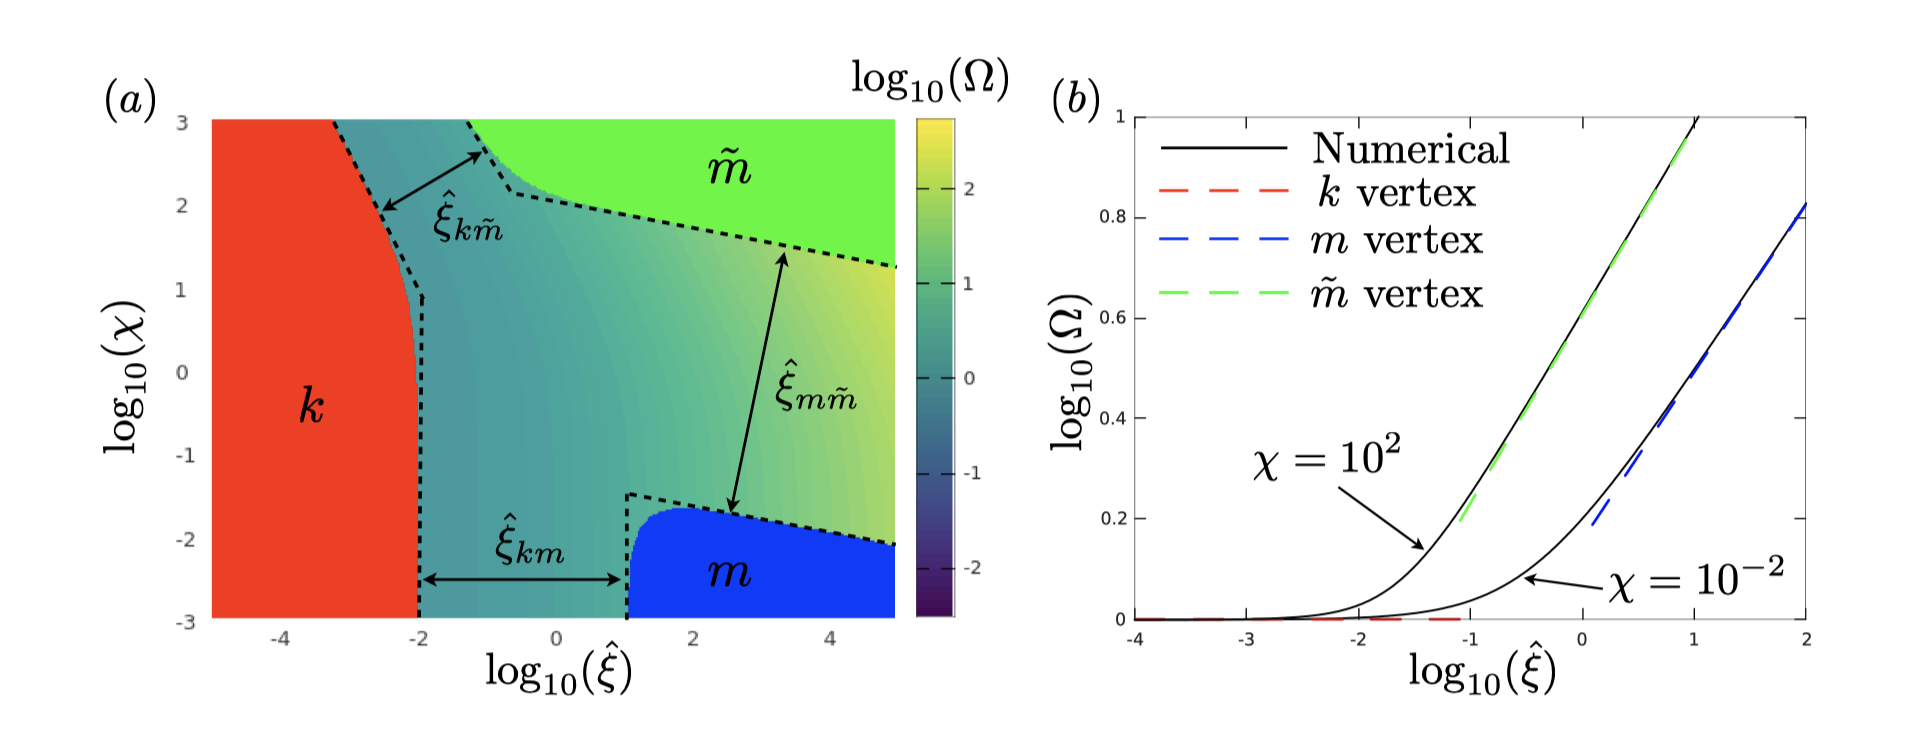
\includegraphics[width=\textwidth]{Dontsov-2021-fig2}
\vspace*{-10mm}
\caption{(a) Параметрическое пространство для задачи моделирования кончика PKN трещины. Цветные области показывают зоны применимости предельных вершинных решений (15) и они также обведены пунктирными чёрными линиями определяемыми выражениями (16). (b) Численное решение зависимости безразмерного раскрытия от безразмерной координаты для двух значений утечки $\chi=10^{-2}$ и $\chi=10^2$ (сплошные черные линии). Вершинные решения (15) показаны пунктирными линиями.}
\label{fig:Dontsov-2021-fig2}
\end{figure}

На рис.2(а) показано численное решение уравнения (14) (вычисленное с использованием явного интегрирования уравнения (14) методом Рунге-Кутты 4-го порядка) в параметрическом пространстве $\left(\hat{\xi},\chi\right)$.
Области применимости асимптотических решений (15) выделены цветными областями.
Эти области определяются как зоны, в которых относительная разница между глобальным решением и соответствующим предельным решением не превышает 1\%.
В частности, красная область соответствует применимости решения трещиностойкости или <<$k$>> решения, синяя область представляет область доминирования вязкости или <<$m$>> решение, а зеленая зона показывает зону применимости решения при доминировании утечек или <<$\tilde{m}$>> решение.
Имеется три переходных области, а именно от $k$ к $m$, от $k$ к $\tilde{m}$ и от $m$ к $\tilde{m}$.
Они оцениваются по следующим параметрам:
\beq
\begin{gathered}
\hat{\xi}_{km}=\hat{\xi},\,\,\,\,\,
\hat{\xi}_{km,1}\approx0.010,\,\,\,\,\,
\hat{\xi}_{km,2}\approx11;\\
\hat{\xi}_{k\tilde{m}}=\hat{\xi}\chi^{2/3},\,\,\,\,\,
\hat{\xi}_{k\tilde{m},1}\approx0.062,\,\,\,\,\,
\hat{\xi}_{k\tilde{m},2}\approx4.4;\\
\hat{\xi}_{m\tilde{m}}=\hat{\xi}\chi^6,\,\,\,\,\,
\hat{\xi}_{m\tilde{m},1}\approx1.85\cdot10^{-8}\,\,\,\,\,
\hat{\xi}_{m\tilde{m},2}\approx2.1\cdot10^{12}.
\end{gathered}
\eeq

Эти параметры вместе с соответствующими им минимальным и максимальным значениями количественно определяют границы применимости предельных вершинных решений и показаны штриховыми черными линиями на рис.2(а).
Простейший способ определить эти переходные параметры состоит в том, чтобы в масштабе приравнять соответствующие вершинные решения, т.е. $\Omega_k\sim\Omega_{\tilde{m}}$ или $1\sim\chi^{1/4}\hat{\xi}^{3/8}$, откуда следует, что $\xi_{k\tilde{m}}=\hat{\xi}\chi^{2/3}$.

На рис. 2(b) показаны линейные графики численного решения, рассчитанного для $\chi=10^{-2}$ и $\chi=10^2$ в зависимости от $\hat{\xi}$ (черные линии).
Штриховыми линиями показаны вершинные решения (15).
Наблюдаются постепенные переходы от решений трещиностойкости к решениям по утечкам или вязкости.

Характерным наблюдением является то, что решение начинается с вершины $k$, затем при некоторых значениях $\chi$ проходит через промежуточную асимптоту $m$, а $\hat{m}$ -- решение в дальней зоне.
Это отличается от классического решения для полубесконечной трещины в условиях плоской деформации, для которого дальнее поле всегда является решением $m$, а $\tilde{m}$ является промежуточным.
Кроме того, учитывая относительно пологий наклон перехода $m\tilde{m}$ в параметрическом пространстве рис.2(a), на практике переход от $m$ к $\tilde{m}$ может быть затруднен.

\begin{figure}[H]
\center
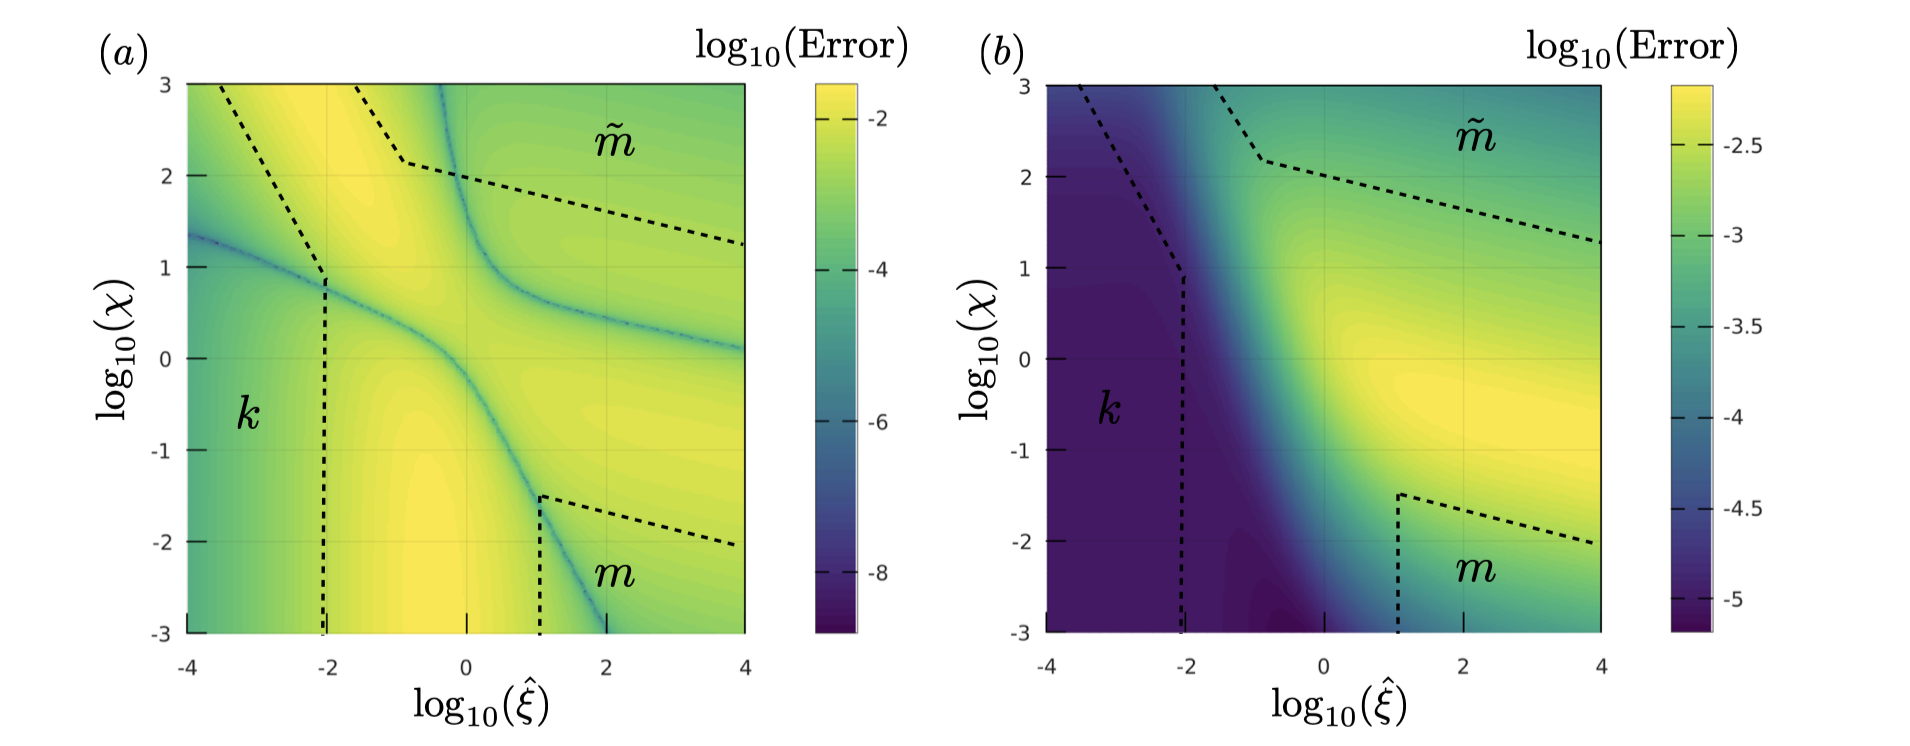
\includegraphics[width=\textwidth]{Dontsov-2021-fig3}
\vspace*{-10mm}
\caption{(a) Относительная ошибка между численным решением и аппроксимациями (11) (рис. (a)) и (12) (рис. (b))}
\label{fig:Dontsov-2021-fig3}
\end{figure}

Для количественной оценки точности аппроксимаций (11) и (12) на рис.3 представлена относительная ошибка между приближенным и численным решениями.
Пространство (а) дает результат для простого решения (11), а пространство (б) соответствует более полному приближению (12).
Максимальная ошибка на всём параметрическом пространстве для первого случая составляет 3\%, а для второго, более точного случая, чуть меньше 0.7\%.
Распределение ошибки также отличается.
Для более простого случая (11) ошибка распределяется примерно равномерно в пределах переходных областей и затухает к пределам вершин.
Во втором случае (12) вершина $k$ и переходы из этой вершины в $m$ и $\tilde{m}$ оказываются заметно точнее, а ошибка возникает в основном в переходе $m\tilde{m}$.
Это неудивительно, поскольку для построения приближения (12) используются точные решения для переходов $km$ и $k\tilde{m}$.

\subsection{Вершинные (асимптотические) решения}

Аналогично задачам о трещинах при условии плоской деформации и радиальных трещинах для геометрии PKN существует четыре предельных решения.
Они определяются конкуренцией между трещиностойкостью и вязкостью, а также накоплением жидкости в трещине и пористой среде.
В частности, определим Storage-Viscosity или предел $М$ как случай, соответствующий преобладанию вязкости и отсутствию утечек, Storage-Toughness или предел $K$ как случай доминирования трещиностойкости и отсутствия утечек, Leak-off-Viscosity или $\tilde{M}$ предел в случае преобладания вязкости и высокой степени утечки, и, наконец, Leak-off-Toughness или предел $\tilde{K}$ в случае преобладания вязкости и высокой степени утечки, см. к примеру обзорную статью [18].\\

\textbf{Storage-Viscosity.}

Для случая Storage-Viscosity основное уравнение (3), граничное условие (5) и баланс объёма (7) сводятся к
\beq
\frac{\partial\bar{w}}{\partial t}-\frac{E'}{2\pi^3\mu H}\frac{\partial^2\bar{w}^4}{\partial x^2}=\frac{Q_0}{H}\delta(x);\,\,\,\,\,
\int\limits_{0}^{l}\bar{w}(x)=\frac{Q_0t}{2H};\,\,\,\,\,
\bar{w}(l)=0.
\eeq

Явным образом включив в глобальное решение поведение вблизи кончика с преобладанием вязкости (9) и ища решение в форме
\beq
\bar{w}=\left(\frac{3\pi^3\mu H}{2E'}\right)^{1/3}\left(\dot{l}\right)^{1/3}l^{1/3}\left(1-\xi\right)^{1/3}f(\xi),\,\,\,\,\,
\xi=\frac{x}{l(t)},
\eeq
баланс объёма в (17) сводится к
\beq
\left(\frac{3\pi^3\mu H}{2E'}\right)^{1/3}\left(\dot{l}\right)^{1/3}l^{4/3}\int\limits_{0}^{1}\left(1-\xi\right)^{1/3}f(\xi)d\xi=\frac{Q_0t}{2H}.
\eeq
Уравновешивая степени $t$ и другие размерные параметры в приведенном выше уравнении, решение для длины можно записать как
\beq
l=c\left(\frac{5E'Q_0^3}{48\pi^3\mu H^4}\right)^{1/5}t^{4/5},
\eeq
где $c$ -- числовая константа, и уравнение баланса объёма принимает вид:
\beq
c^{5/3}\int\limits_{0}^{1}\left(1-\xi\right)^{1/3}f(\xi)d\xi=1.
\eeq

С приведенным выше определением ширины (18) и длины (20) уравнение Рейнольдса в (17) преобразуется в
\beq
\frac{1}{4}\left(1-\xi\right)^{1/3}f(\xi)-\xi\frac{d(1-\xi)^{1/3}f(\xi)}{d\xi}-\frac{3}{4}\frac{d^2(1-\xi)^{4/3}(f(\xi))^4}{d\xi^2}=0
\eeq
с граничными условиями
\beq
-c^{5/3}\frac{3}{5}\frac{d(1-\xi)^{4/3}f^4}{d\xi}\bigg|_{\xi=0}=1,\,\,\,\,\,
f|_{\xi=1}=1.
\eeq

Вместо решения дифференциального уравнения (22) решение ищется в виде $f=1+a\left(1-\xi\right)$, т.е. разлагая его вблизи кончика.
Подставляя этот результат в (22) и уравновешивая степени $\left(1-\xi\right)$, предполагая, что последний является малым параметром, получается $a=-1/96$.
Это показывает, что линейная поправка к решению на кончике (т. е. $f=1$) составляет порядка 1\% даже вблизи источника.
Поэтому представляется достаточным рассмотреть только линейный член и записать приближенное решение для $f$ в виде
\beq
f(\xi)\approx1-\frac{1-\xi}{96}.
\eeq

Подставляя (24) в (21), числовой коэффициент $c$ принимает вид
\beq
c=\left(\frac{224}{167}\right)^{3/5}\approx1.193.
\eeq

Подводя итог, приближенное вершинное решение $M$ вычисляется с использованием (18), (20), (24) и (25) как
\beq
\begin{gathered}
\bar{w}_M=1.76\left(\frac{\mu Q_0^2}{E'H}\right)^{1/5}t^{1/5}(1-\xi)^{1/3}\left(1-\frac{1-\xi}{96}\right),\\
p_M=1.12\left(\frac{\mu E'^4Q_0^2}{H^6}\right)^{1/5}t^{1/5}(1-\xi)^{1/3}\left(1-\frac{1-\xi}{96}\right),\\
l_M=0.38\left(\frac{E'Q_0^3}{\mu H^4}\right)^{1/5}t^{4/5}.
\end{gathered}
\eeq

Здесь уравнение локальной упругости (1) используется для вычисления давления.
Заметим, что это приближенное решение основано главным образом на поведении вблизи кончика, а условие на входе (23) не выполняется.
Поэтому вблизи входа могут быть некоторые расхождения с <<истинным>> решением.
Эти выражения совпадают с приведенными в [1] с точностью до нескольких процентов. Это приемлемое отличие, поскольку для вывода выражений, представленных в [1], также используются аппроксимации.\\

\textbf{Leak-off-Viscosity.}

Для случая Leak-off-Viscosity трещиностойкость и объем трещины пренебрежимо малы.
В результате определяющее уравнение (3), граничное условие (5) и глобальный баланс объёма (7) сводятся к
\beq
-\frac{E'}{2\pi^3\mu H}\frac{\partial^2\bar{w}^4}{\partial x^2}+\frac{C'}{\sqrt{t-t_0(x)}}=\frac{Q_0}{H}\delta(x),\,\,\,\,\,
2C'\int\limits_0^l\sqrt{t-t_0(x)}dx=\frac{Q_0t}{2H},\,\,\,\,\,
\bar{w}(l)=0.
\eeq
Приняв зависимость длины от времени как $l\propto t^{\alpha}$, время воздействия, необходимое для расчёта утечки становится равным $t_0(x)=t(x/l)^{1/\alpha}$.
В этом случае глобальный баланс объёма сводится к
\beq
2C't^{1/2}l\int\limits_0^1\sqrt{1-\xi^{1/\alpha}}d\xi=\frac{Q_0t}{2H}.
\eeq

Уравновешивая степени $t$ в приведенном выше выражении, получаем $\alpha=1/2$, а длина равна
\beq
l=\frac{Q_0t^{1/2}}{\pi C'H}.
\eeq

Зная выражение для $t_0(x)$, уравнение Рейнольдса в (27) сводится к виду
\beq
-\frac{E'}{2\pi^3\mu H}\frac{\partial^2\bar{w}^4}{\partial x^2}+\frac{C'}{\sqrt{t}\sqrt{1-(x/l)^2}}=\frac{Q_0}{H}\delta(x),\,\,\,\,\,
\bar{w}(l)=0,
\eeq
которое можно решить и получить
\beq
\bar{w}=\left(\frac{2\pi\mu Q_0^2}{E'C'H}\right)^{1/4}t^{1/8}g(\xi);\,\,\,\,\,
g(\xi)=\left[\xi\left(\sin^{-1}{\left(\xi\right)}-\frac{\pi}{2}\right)+\sqrt{1-\xi^2}\right]^{1/4};\,\,\,\,\,
\xi=\frac{x}{l}.
\eeq
Наконец решение для вершины $\tilde{M}$ можно обобщить как
\beq
\begin{gathered}
\bar{w}_{\tilde{M}}=\left(\frac{2\pi\mu Q_0^2}{E'C'H}\right)^{1/4}t^{1/8}g(\xi),\\
p_{\tilde{M}}=\left(\frac{32\mu E'^3Q_0^2}{\pi^3C'H^5}\right)^{1/4}t^{1/8}g(\xi),\\
l_{\tilde{M}}=\frac{Q_0t^{1/2}}{\pi C'H}
\end{gathered}
\eeq
где функция $g(\xi)$ определена в (31).
Это решение в точности совпадает с решением [1].

Отметим, что функция $g(\xi)$, определённая в (31), имеет следующую асимптотику:
\beq
g(\xi)|_{\xi\to1}=\left(\frac{8}{9}\right)^{1/8}\left(1-\xi\right)^{3/8},\,\,\,\,\,g(0)=1.
\eeq
Учитывая, что $(8/9)^{1/8}\approx0.985$, т.е. близка к единице, функция $g$ может быть аппроксимирована через её асимптотическое поведение как
\beq
g(\xi)\approx\left(\frac{8}{9}\right)^{1/8}\left(1-\xi\right)^{3/8}\left[1-\left(1-\left(\frac{9}{8}\right)^{1/8}\right)\left(1-\xi\right)\right].
\eeq
Эта форма решения для ширины трещины очень похожа на решение Storage-Viscosity (26).
Общим также является то, что множитель перед <<поправочным членом>> $\left(1-\xi\right)$  относительно мал, порядка 1\%.\\

\textbf{Storage-Toughness.}

В пределе отсутствия вязкости и отсутствия утечек весь закачиваемый объем остается внутри трещины и отсутствует градиент давления вдоль трещины.
Вследствие постоянного давления и локальной упругости ширина трещины в этом пределе постоянна.
Комбинация граничного условия (5) и баланса объемов (7) приводит к решению в виде
\beq
\begin{gathered}
\bar{w}_K=\frac{K_{Ic}\sqrt{\pi H}}{E'},\\
p_K=\frac{2K_{Ic}}{\sqrt{\pi H}},\\
l_K=\frac{E'Q_0t}{\sqrt{4\pi}K_{Ic}H^{3/2}}.
\end{gathered}
\eeq

\textbf{Leak-off-Toughness.}

В пределе доминирования трещиностойкости ширина и давление постоянны вдоль трещины и определяются исключительно граничным условием на кончике (5), как и в предыдущем случае.
Разница возникает из-за баланса объема, в котором нагнетаемая жидкость теперь уравновешивается утечкой, а именно
\beq
\int\limits_{0}^{l}{2C'\sqrt{t-t_0(x)}dx}=\frac{Q_0t}{2H}.
\eeq

Аналогично случаю Leak-off-Viscosity, приняв зависимость длины от времени как $l\propto t^{\alpha}$, получим $t_0(x)=t(x/l)^{1/\alpha}$, и в этом случае приведенный выше интеграл сводится к
\beq
2C't^{1/2}l\int\limits_{0}^{1}{\sqrt{1-\xi^{1/\alpha}}d\xi}=\frac{Q_0t}{2H}.
\eeq

Уравновешиваем степени $t$ и становится ясно, что $\alpha=1/2$.
В результате приведенное выше уравнение позволяет найти $l$, что в сочетании с выражениями для ширины и давления, вытекающими из граничного условия, дает следующий результат
\beq
\begin{gathered}
\bar{w}_{\tilde{K}}=\frac{K_{Ic}\sqrt{\pi H}}{E'},\\
p_{\tilde{K}}=\frac{2K_{Ic}}{\sqrt{\pi H}},\\
l_{\tilde{K}}=\frac{Q_0t^{1/2}}{\pi C' H}.
\end{gathered}
\eeq

Интересно отметить, что разница этого результата с предыдущим решением Storage-Toughness заключается только в длине трещины, в то время как ширина и давление точно такие же.
С другой стороны, длина такая же, как и для предела Leak-off-Viscosity.


\subsection{Полное решение}

Этот раздел направлен на построение и анализ полного решения модели трещины PKN, которое включает эффекты трещиностойкости, вязкости и утечки.
Построены два типа решений: полуаналитическое быстрое приближенное решение и полностью численное решение.
Первое позволяет быстро вычислить решение и исследовать всё параметрическое пространство, а второе позволяет проверить точность аппроксимации.

Как видно из предельных вершинных решений (26), (32), (35) и (38), пространственное изменение ширины трещины хорошо аппроксимируется соответствующими вершинными асимптотами (9).
Существует некоторое расхождение для решений Storage-Viscosity и Leak-off-Viscosity, но оно составляет порядка 1\% и поэтому для простоты игнорируется.
Исходя из этого наблюдения, ширина в глобальном решении принимается в виде:
\beq
\bar{w}=\bar{w}_{m\tilde{m}k}\left(\hat{x}=l\left(1-\xi\right),V=\dot{l}\right),\,\,\,\,\,
\xi=\frac{x}{l},
\eeq
где $\bar{w}_{m\tilde{m}k}$ -- приближенное решение для полубесконечной трещины (12), которое также зависит от $E'$, $K_{Ic}$, $\mu$, $C'$ и $H$.
Отметим, что подход к построению глобального решения из асимптотического решения для кончика был применен в [25] для радиальной трещины и в [26] для трещины в условиях плоской деформации.
Одним из заметных отличий для трещины PKN является тот факт, что асимптота кончика прерывиста на кончике и, следовательно, не очень точно аппроксимировать пространственное поведение с помощью $\left(1-\xi\right)^{\delta}$ (с медленно меняющейся функцией $\delta$), как это было сделано в предыдущих случаях.
Для построения глобального решения по (39) необходимо также учитывать глобальный баланс объёма (7).
Приняв $l\propto t^{\alpha}$, где $\alpha$ -- медленно меняющаяся функция времени, время воздействия утечки принимает вид $t_0(x)=t(x/l)^{1/\alpha}$ и баланс объёма (7) сводится к
\beq
l\int\limits_{0}^{1}{\bar{w}_{m\tilde{m}k}}\left(l\left(1-\xi\right),\alpha l/t\right)d\xi+2C't^{1/2}l\int\limits_{0}^{1}{\sqrt{1-\xi^{1/\alpha}}}d\xi=\frac{Q_0t}{2H}.
\eeq

Интеграл, связанный с утечкой, в приведенном выше уравнении может быть вычислен аналитически, что приводит к следующей системе уравнений
\beq
l\int\limits_{0}^{1}{\bar{w}_{m\tilde{m}k}}\left(l\left(1-\xi\right),\alpha l/t\right)d\xi+\sqrt{\pi}C't^{1/2}l\frac{\Gamma(\alpha+1)}{\Gamma(\alpha+\frac{3}{2})}=\frac{Q_0t}{2H},\,\,\,\,\,\,\,\,\,\,
\alpha=\frac{d\log(l)}{d\log(t)}
\eeq
где $\Gamma(\cdot)$ обозначает гамма-функцию.
Интеграл ширины трещины в приведенном выше выражении вычисляется численно.
Поскольку $\alpha$ меняется медленно, первое уравнение можно решить итеративно для $l$, например используя метод Ньютона.
Как только длина $l$ вычисляется для двух моментов времени, значение $\alpha$ обновляется.
Такие итерации продолжаются до тех пор, пока не будет достигнута сходимость.
Как только эти величины вычислены, решение по ширине оценивается с помощью (39), а давление всегда можно вычислить с помощью (1).

Для численного решения рассматриваемой задачи, как и в предыдущем случае, вводится подвижная координата $\xi=x/l(t)$.
Для дальнейшего упрощения задачи используется следующая нормализация
\beq
\Omega=\frac{\bar{w}}{w_{*}},\,\,\,\,\,
\lambda=\frac{l}{l_{*}},\,\,\,\,\,
\tau=\frac{t}{t_{*}},
\eeq
где масштабы ширины, длины и времени задаются следующими формулами:
\beq
w_{*}=\frac{\left(\pi H\right)^{1/2}K_{Ic}}{E'},\,\,\,\,\,
l_{*}=\frac{H^2K_{Ic}^4}{2\pi E'^3\mu Q_0},\,\,\,\,\,
t_{*}=\frac{H^{7/2}K_{Ic}^5}{2\pi^{1/2}E'^4\mu Q_0^2}.
\eeq

При такой нормировке основные уравнения (3), (5) и (6) сводятся к
\beq
\frac{\partial\Omega}{\partial\tau}-\frac{\xi\dot{\lambda}}{\lambda}\frac{\partial\Omega}{\partial\xi}-\frac{1}{\lambda^2}\frac{\partial^2\Omega^4}{\partial\xi^2}+\frac{\phi}{\sqrt{\tau-\tau_0(\xi)}}=\delta(\xi),\,\,\,\,\,
\Omega(1)=1,\,\,\,\,\,
\frac{d\lambda}{d\tau}=-\frac{4}{3\lambda}\frac{\partial\Omega^3}{\partial\xi}\bigg|_{\xi=1}.
\eeq
Здесь безразмерный параметр, описывающий утечку, рассчитывается как
\beq
\phi=\left(\frac{H^5K_{Ic}^6C'^4}{4\pi^3E'^4\mu^2Q_0^4}\right)^{1/4}
\eeq
Решение приведенной выше безразмерной задачи (44) состоит в нахождении $\Omega(\tau,\phi)$ и $\lambda(\tau)$.
После решения безразмерной задачи физические величины можно восстановить с помощью (42) и (43).
Это свидетельствует о том, что параметрическое пространство для задачи является двумерным и состоит из безразмерного времени $\tau$ и безразмерной утечки $\phi$, что в чем-то аналогично случаю радиальной трещины [25].
Численное решение задачи (44) вычисляется с использованием центральной разности для дискретизации пространственных производных и обратной разности для аппроксимации производной по времени для обеспечения устойчивости численной схемы.

\begin{figure}[H]
\center
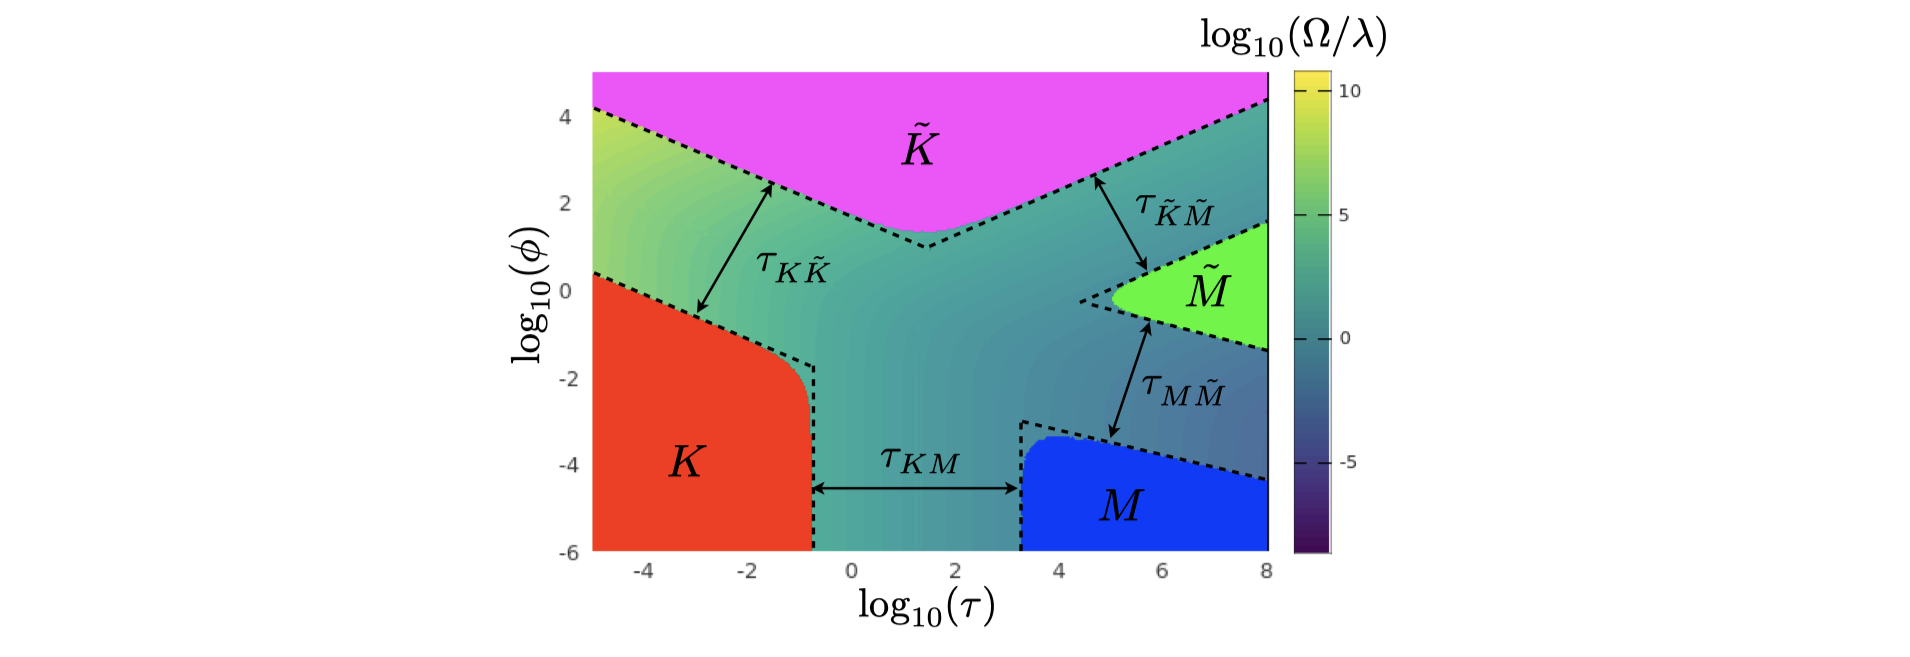
\includegraphics[width=\textwidth]{Dontsov-2021-fig4}
\vspace*{-10mm}
\caption{Параметрическое пространство для трещины PKN. Зоны применимости предельных вершинных решений выделены красным ($K$ или Storage-Toughness), синим ($M$ или Storage-Viscosity), пурпурным ($\tilde{K}$ или Leak-off-Toughness) и зелёным ($\tilde{M}$ или Leak-off-Viscosity)}
\label{fig:Dontsov-2021-fig4}
\end{figure}

На рис.4 показано параметрическое пространство для рассматриваемой задачи, вычисляемое с помощью быстрого приближенного решения (41).
В частности, решение строится в пространстве $(\tau,\phi)$ в терминах отношения $\Omega/\lambda$ (см. (42), (43), (45)).
Это делается для того, чтобы отображаемая величина была разной для всех предельных случаев.
Зоны применимости предельных вершинных решений обозначены красной, синей, пурпурной и зеленой областями.
Последние определяются как области, в которых разница $\Omega/\lambda$ с соответствующим вершинным решением меньше 1\%.
Красная область соответствует решению Storage-Toughness (35), синяя область представляет предел Storage-Viscosity (26), пурпурная область определяет предел Leak-off-Toughness (38), а зеленая область соответствует решению Leak-off-Viscosity (32).
Штриховыми линиями на рис.4 обозначены зоны применимости вершинных решений.
Чтобы получить соответствующий параметр, определяющий переход, необходимо приравнять либо длину, либо ширину (в зависимости от того, что отличается) между двумя режимами.
Например, переход между $K$ и $M$ определяется параметром, вычисляемым из $l_{M}\sim l_{K}$ или $\bar{w}_{M}\sim\bar{w}_{K}$.
Для количественной оценки параметра перехода $\tilde{K}K$ следует использовать $l_{\tilde{K}}\sim l_K$.
Ширина не может быть использована, так как они для обоих режимов идентичны.
Аналогично, для перехода $\tilde{K}\tilde{M}$ необходимо использовать ширину $\bar{w}_{\tilde{K}}\sim\bar{w}_{\tilde{M}}$, поскольку длины одинаковы.
Наконец, для $M\tilde{M}$ можно использовать либо ширину, либо длину, т. е. $l_M\sim l_{\tilde{M}}$ или $\bar{w}_M\sim\bar{w}_{\tilde{M}}$.
Значения параметров перехода определяются численно.
Сводка результатов показана ниже:
\beq
\begin{gathered}
\tau_{MK}=\tau,\,\,\,\,\,\,
\tau_{MK,1}=0.11,\,\,\,\,\,\,
\tau_{MK,2}=2.3\cdot10^3,\\
\tau_{K\tilde{K}}=\tau\phi^2,\,\,\,\,\,\,
\tau_{K\tilde{K},1}=5.7\cdot10^{-5},\,\,\,\,\,\,
\tau_{K\tilde{K},2}=3.1\cdot10^3,\\
\tau_{\tilde{K}\tilde{M}}=\tau\phi^{-2},\,\,\,\,\,\,
\tau_{\tilde{K}\tilde{M},1}=0.18,\,\,\,\,\,\,
\tau_{\tilde{K}\tilde{M},2}=6.5\cdot10^4,\\
\tau_{M\tilde{M}}=\tau\phi^{10/3},\,\,\,\,\,\,
\tau_{M\tilde{M},1}=2.0\cdot10^{-7},\,\,\,\,\,\,
\tau_{M\tilde{M},2}=2.9\cdot10^3.
\end{gathered}
\eeq
Обратите внимание, что определения зон применимости предельных решений несколько произвольны, и результат может измениться, если используется другая метрика или другое пороговое значение.
Кроме того, может быть небольшое несоответствие, так для построения параметрической карты используется приближённое решение.
В то же время, поскольку параметрическое пространство построено в логарифмическом масштабе, незначительные изменения границ, определяемых (46), не должны заметно изменить результат.

В полученном результате интересно то, что трещина развивается во времени от вершины $K$ и в конечном итоге достигает вершины $\tilde{M}$.
Оно может пройти через $\tilde{K}$, $M$ или ни через одно из них в промежуточные моменты времени.
Это несколько противоположно геометрии радиальной трещины, для которой решение всегда исходит из вершины $M$, а затем достигает решения $\tilde{K}$ в долгосрочной перспективе.
Это также отличается от трещины в условиях плоской деформации, для которой решение начинается на краю $MK$ и в конечном итоге достигает края $\tilde{M}\tilde{K}$.

\begin{figure}[H]
\center
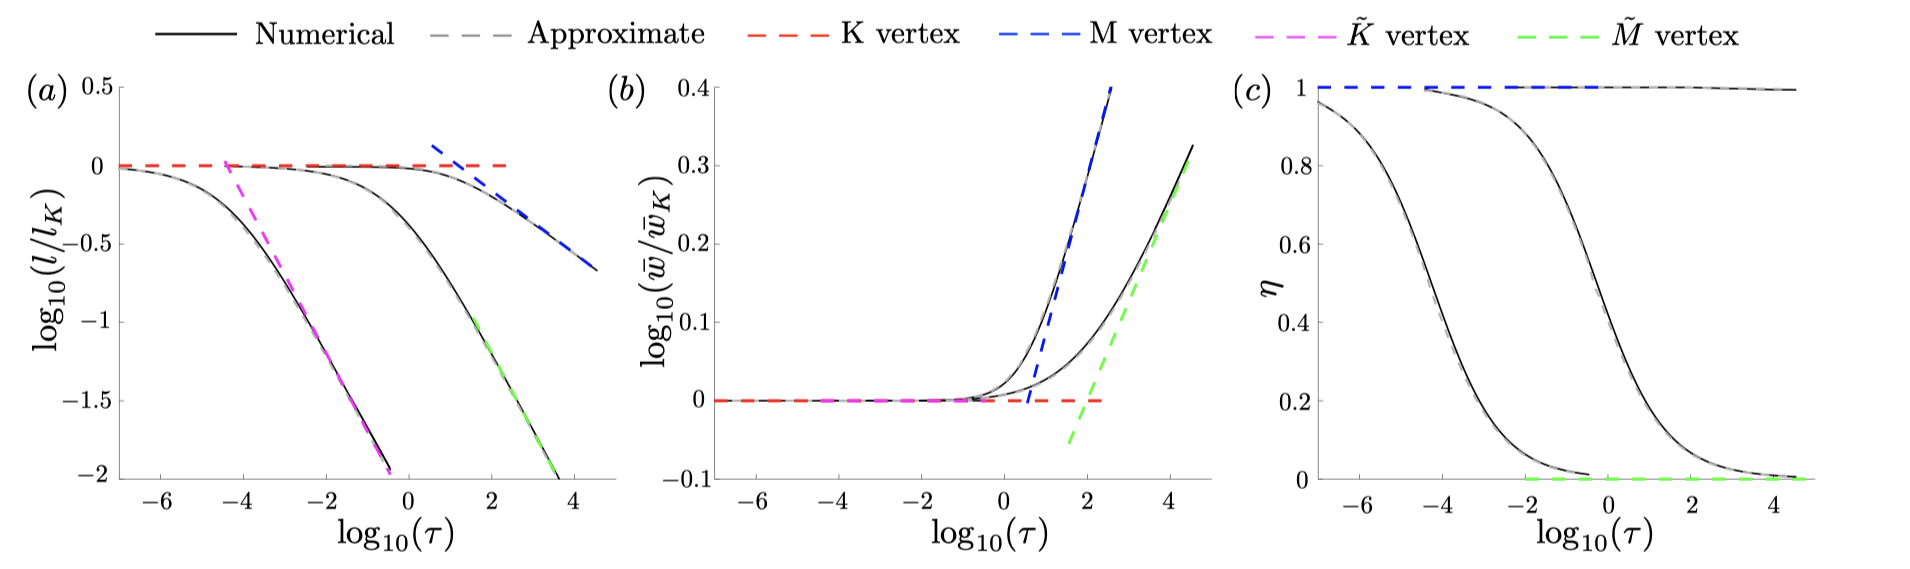
\includegraphics[width=\textwidth]{Dontsov-2021-fig5}
\vspace*{-10mm}
\caption{Сравнение между численным, приближённым и вершинным решениями для трёх значений параметра безразмерных утечек $\phi=\{10^{-4},1,10^2\}$. (a) Нормализованная длина трещины в зависимости от времени. (b) Нормализованная ширина трещины около скважины в зависимости от времени. (c) Эффективность в зависимости от времени.}
\label{fig:Dontsov-2021-fig5}
\end{figure}

\begin{figure}[H]
\center
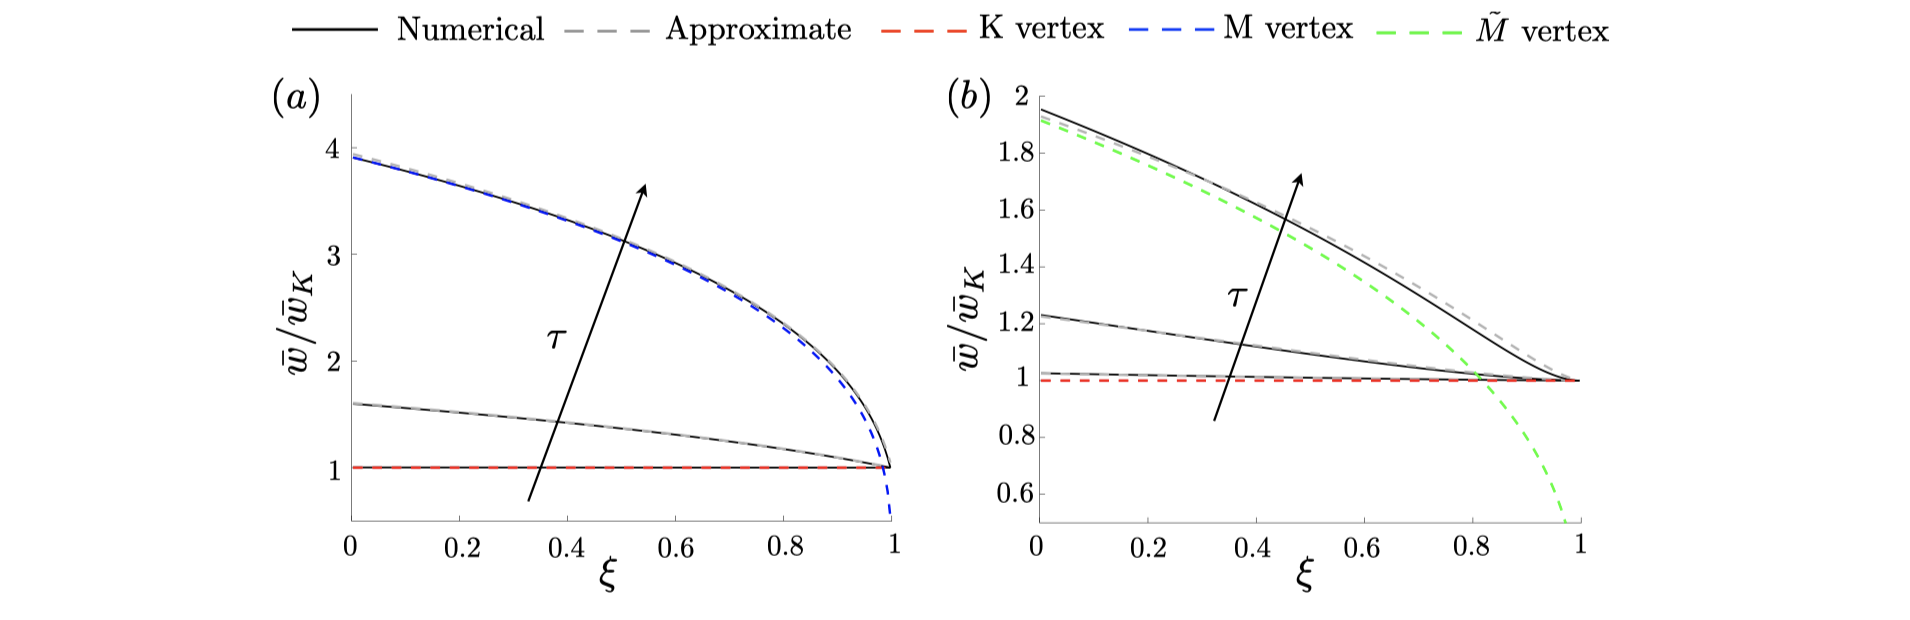
\includegraphics[width=\textwidth]{Dontsov-2021-fig6}
\vspace*{-10mm}
\caption{Сравнение между численным, приближённым и вершинным решениями в терминах изменения ширины трещины в зависимости от нормализованной пространственной координаты $\xi$. (a) Соответствует значениям параметров $\phi=10^{-4}$ и $\tau=\sqrt{4\pi}\{10^{-2},10,10^3\}$. (b) Соответствует значениям $\phi=1$ и $\tau=\sqrt{4\pi}\{0.5,50,5\cdot10^3\}$}
\label{fig:Dontsov-2021-fig6}
\end{figure}

Также поучительно проверить, что решение, построенное с использованием асимптоты на кончике и баланса объёма, точно аппроксимирует численное решение.
На рис.4 три значения параметра утечки выбраны $\phi=\{10^{-4},1,10^2\}$.
Эти три значения $\phi$ позволяют исследовать переходы от решения $K$ к другим трём вершинам.
На рис.5 показано сравнение между численным решением (сплошные чёрные линии) и приближённым решением (пунктирные серые линии) через изменение нормированной длины трещины $l/l_K$, ширины в стволе скважины $w/w_K$ и эффективности $\eta$, где последняя определяется как отношение объема трещины к закачиваемому объему.
Вершинные решения показаны пунктирными цветными линиями.
Можно заметить, что решение действительно переходит из предела $K$ в предел $M$, $\tilde{M}$ или $\tilde{K}$.
Кроме того, приближенное решение визуально почти неотличимо от решения, рассчитанного численно.
Для дальнейшего сравнения двух решений на рис.6 показано нормированное изменение ширины трещины вдоль её длины для $\phi=10^{-4}$ и $\tau=\sqrt{4\pi}\{10^{-2},10,10^3\}$], а также для $\phi=1$ и $\tau=\sqrt{4\pi}\{0.5,50,5\cdot10^3\}$.
Заметим, что случай, соответствующий $\phi=10^2$, тривиален, так как ширина для этого перехода постоянна.
Результаты снова показывают, что разница между численным и приближенным решениями невелика.
Таким образом, подтверждается, что параметрическое пространство, вычисленное с помощью быстрого приближенного решения, построено с достаточной степенью точности.

\subsection{Примеры применения}

Чтобы проиллюстрировать полученные результаты, в этом разделе представлены два примера того, как параметрическая карта может использоваться в приложениях.

Сначала рассмотрим полевой случай с параметрами $H=20\text{ м}$, $K_{Ic}=1\text{ МПа}\cdot\text{м}^{1/2}$, $C'=10^{-6}\text{ м}/\text{с}^{1/2}$, $E'=30\text{ ГПа}$, $\mu=0.01\text{ Па}\cdot\text{с}$, $Q=0.01\text{ м}^3/\text{с}$, $t=1000\text{ с}$.
Из выражений (42), (43) и (45) безразмерные параметры для этого случая равны $\tau\approx8\cdot10^4$ и $\phi\approx4\cdot10^{-4}$.
Глядя на параметрическую карту на рис.4, можно сделать вывод, что решение соответствует случаю с преобладанием Storage-Viscosity.
Следовательно, длина трещины может быть рассчитана из выражения (26) и равна $l\approx170\text{ м}$.

Во-вторых, рассмотрим параметры, используемые в [40] для оценки производительности различных численных алгоритмов в режиме трещиностойкости.
Соответствующие параметры взяты из лабораторных экспериментов и равны $H=0.05\text{ м}$, $K_{Ic}=1.57\text{ МПа}\cdot\text{м}$, $C'=0\text{ м}/\text{с}^{1/2}$, $E'=3.9\text{ ГПа}$, $\mu=30.2\text{ Па}\cdot\text{с}$, $Q=1.7\text{мм}^3/\text{с}$, $t=604\text{с}$.
Согласно уравнениям (42), (43) и (45) безразмерные параметры для этого случая равны $\tau=0.2$ и $\phi=0$.
Эти параметры попадают в режим Storage-Toughness на параметрической карте, представленной на рис.4.
Таким образом, это подтверждает, что в [40] действительно сравниваются разные алгоритмы в режиме трещиностойкости.
Наконец, уравнение (35) можно использовать для расчета длины трещины и эта длина равна $6.5\text{ см}$, что также согласуется с численными результатами, представленными в [40].

\subsection{Резюме}

В данной работе исследована задача трещины гидроразрыва постоянной высоты или трещины PKN.
Рассмотрены комбинированные эффекты трещиностойкости, вязкости жидкости и утечек.
Кроме того, для уменьшения сложности анализа вместо более точного соотношения нелокальной упругости используется локальная упругость.

Сначала намечается анализ проблемы для области кончика трещины.
Показано, что, как и в классическом случае полубесконечной трещины в условиях плоской деформации, существует три предельных или вершинных решения, связанных с преобладанием либо трещиностойкости, либо вязкости, либо утечек.
Получена параметрическая карта решений, в которой очерчены зоны применимости предельных решений.
Кроме того, строятся два приближенных решения задачи и оценивается их точность во всем параметрическом пространстве.

Для конечной трещины PKN сначала получаются явные выражения для четырех предельных решений.
Эти пределы имеют то же значение, что и пределы для других геометрий трещины ГРП, таких как трещина в условиях плоской деформации и радиальная трещина, и включают пределы Storage-Viscosity, Storage-Toughness, Leak-off-Viscosity и Leak-off-Toughness.
Полное решение для конечной трещины PKN вычисляется с использованием двух подходов: численного решения и быстрого приближения.
Последний использует развитое асимптотическое решение на кончике в качестве аппроксимации пространственного изменения ширины всей трещины.
Этот подход в сочетании с глобальным балансом объема позволил построить быстрое решение проблемы.
Точность этого приближения оценивается путем сравнения его предсказаний с предсказаниями численного решения.
С помощью этого быстрого решения исследуется всё параметрическое пространство задачи и намечаются зоны применимости предельных решений.
Одно интересное наблюдение состоит в том, что глобальное решение эволюционирует от предела Storage-Toughness на раннем этапе до предела Leak-off-Viscosity на поздних временах.
Это отличается от поведения для ранее проанализированных геометрий радиальной трещины и плоской трещины.
Полученные результаты позволяют легко оценить положение внутри параметрического пространства при любых входных параметрах задачи для трещины постоянной высоты, что может быть использовано, например, для приведения промысловых данных к лабораторному эксперименту или использования ближайшего предельного решения для оценки геометрии трещины ГРП.

\subsection*{Список использованной литературы}
\addcontentsline{toc}{subsection}{Список использованной литературы}

[1] M.J. Economides and K.G. Nolte, editors. Reservoir Stimulation. John Wiley \& Sons, Chichester, UK, 3rd edition, 2000.

[2] E. Detournay and D. Garagash. The tip region of a fluid-driven fracture in a permeable elastic solid. J.Fluid Mech., 494:1–32, 2003.

[3] D.I. Garagash, E. Detournay, and J.I. Adachi. Multiscale tip asymptotics in hydraulic fracture with leak-off. J. Fluid Mech., 669:260–297, 2011.

[4] A. Peirce and E. Detournay. An implicit level set method for modeling hydraulically driven fractures. Comput. Methods Appl. Mech. Engrg., 197:2858–2885, 2008.

[5] J. Desroches, E. Detournay, B. Lenoach, P. Papanastasiou, J.R.A. Pearson, M. Thiercelin, and A.H.-D. Cheng. The crack tip region in hydraulic fracturing. Proc. R. Soc. Lond. A, 447:39–48, 1994.

[6] B. Lenoach. The crack tip solution for hydraulic fracturing in a permeable solid. J. Mech. Phys. Solids, 43:1025–1043, 1995.

[7] J.R. Rice. Mathematical analysis in the mechanics of fracture. In H. Liebowitz, editor, Fracture: An Advanced Treatise, volume II, chapter 3, pages 191–311. Academic Press, New York, NY, 1968.

[8] E. Dontsov and A. Peirce. A non-singular integral equation formulation to analyze multiscale behaviour in semi-infinite hydraulic fractures. J. Fluid. Mech., 781:R1, 2015.

[9] E.V. Dontsov and A.P. Peirce. A multiscale implicit level set algorithm (ILSA) to model hydraulic fracture propagation incorporating combined viscous, toughness, and leak-off asymptotics. Comput. Methods Appl. Mech. Engrg., 313:53–84, 2017.

[10] E.V. Dontsov and O. Kresse. A semi-infinite hydraulic fracture with leak-off driven by a power-law fluid. J. Fluid Mech., 837:210–229, 2018.

[11] A.O. Bessmertnykh, E.V. Dontsov, and R. Ballarini. A semi-infinite hydraulic fracture driven by a Herschel-Bulkley fluid. J. Appl. Mech., 86:121008, 2019.

[12] F.-E. Moukhtari and B. Lecampion. A semi-infinite hydraulic fracture driven by a shear-thinning fluid. Journal of Fluid Mechanics, 838:573–605, 2018.

[13] D. Garagash and E. Detournay. The tip region of a fluid-driven fracture in an elastic medium. J. Appl. Mech., 67:183–192, 2000.

[14] E.V. Dontsov. Tip region of a hydraulic fracture driven by a laminar-to-turbulent fluid flow. J. Fluid. Mech., 797:R2, 2016.

[15] D.I. Garagash. Cohesive-zone effects in hydraulic fracture propagation. Journal of the Mechanics and Physics of Solids, 133:103727, 2019.

[16] A. Bessmertnykh, E. Dontsov, and R. Ballarini. The effects of proppant on the near-front behavior of a hydraulic fracture. Engineering Fracture Mechanics, page 107110, 2020.

[17] E.A. Kanin, D.I. Garagash, and A.A. Osiptsov. The near-tip region of a hydraulic fracture with pressure-dependent leak-off and leak-in. Journal of Fluid Mechanics, 892:A31, 2020.

[18] E. Detournay. Mechanics of hydraulic fractures. Annu. Rev. Fluid Mech., 48:31139, 2016.

[19] A. Savitski and E. Detournay. Similarity solution of a penny-shaped fluid-driven fracture in a zerotoughness linear elastic solid. CR. Acad. Sci. II B, 329:255–262, 2001.

[20] J.I. Adachi and E. Detournay. Self-similar solution of a plane-strain fracture driven by a power-law fluid. Int. J. Numer. Anal. Meth. Geomech., 26:579–604, 2002.

[21] A. Bunger, E. Detournay, and D. Garagash. Toughness-dominated hydraulic fracture with leak-off. Int. J. Fract., 134:175–190, 2005.

[22] J. I. Adachi and E. Detournay. Plane-strain propagation of a hydraulic fracture in a permeable rock. Engng Fract. Mech., 75:4666–4694, 2008.

[23] J. Hu and D.I. Garagash. Plane-strain propagation of a fluid-driven crack in a permeable rock with fracture toughness. J. Eng. Mech., 136:1152–1166, 2010.

[24] M.V. Madyarova. Fluid-driven penny-shaped fracture in elastic medium. Master’s thesis, University of Minnesota, 2003.

[25] E.V. Dontsov. An approximate solution for a penny-shaped hydraulic fracture that accounts for fracture toughness, fluid viscosity, and leak-off. R. Soc. open sci., 3:160737, 2016.

[26] E.V. Dontsov. An approximate solution for a plane strain hydraulic fracture that accounts for fracture toughness, fluid viscosity, and leak-off. Int. J. Fract., 205:221–237, 2017.

[27] E.V. Dontsov. Scaling laws for hydraulic fractures driven by a power-law fluid in homogeneous anisotropic rocks. Int. J. Numer. Anal. Methods Geomech., 43:519–529, 2019.

[28] E. Dontsov, A. Bunger, B. Abell, and R. Suarez-Rivera. Ultrafast hydraulic fracturing model for optimizing cube development. In Proceedings of the Unconventional Resources Technology Conference, doi:10.15530/urtec-2019-884, 2019.

[29] T.K. Perkins and L.R. Kern. Widths of hydraulic fractures. J. Pet. Tech. Trans. AIME, pages 937–949, 1961.

[30] R.P. Nordgren. Propagation of vertical hydraulic fractures. Soc. Petrol. Eng. J., pages 306–314, 1972.

[31] A. Settari and M.P. Cleary. Development and testing of a pseudo-three-dimensional model of hydraulic fracture geometry (p3dh). In Proceedings of the 6th SPE symposium on reservoir simulation of the Society of Petroleum Engineers, SPE 10505, pages 185–214, 1986.

[32] J. I. Adachi, E. Detournay, and A. P. Peirce. An analysis of classical pseudo-3D model for hydraulic fracture with equilibrium height growth across stress barriers. Int. J. of Rock Mech. and Min. Sci., 47:625–639, 2010.

[33] E. Dontsov and A. Peirce. An enhanced pseudo-3D model for hydraulic fracturing accounting for viscous height growth, non-local elasticity, and lateral toughness. Eng. Frac. Mech., 142:116–139, 2015.

[34] Y. Kovalyshen and E. Detournay. A reexamination of the classical PKN model of hydraulic fracture. Transp Porous Med, 81:317–339, 2010.

[35] P. Xing, K. Yoshioka, J. Adachi, A. El-Fayoumi, and A. P. Bunger. Laboratory measurement of tip and global behavior for zero-toughness hydraulic fractures with circular and blade-shaped (PKN) geometry. Journal of the Mechanics and Physics of Solids, 104:172–186, 2017.

[36] N. Zolfaghari, C. R. Meyer, and A. P. Bunger. Blade-shaped hydraulic fracture driven by a turbulent fluid in an impermeable rock. Journal of Engineering Mechanics, 143(11):04017130, 2017.

[37] H. Zia and B. Lecampion. Propagation of a height contained hydraulic fracture in turbulent flow regimes. International Journal of Solids and Structures, 110-111:265–278, 2017.

[38] K.G. Nolte. Fracturing-pressure analysis for nonideal behavior. J. Pet. Technol., 43:210–218, 1991.

[39] E. Sarvaramini and D. Garagash. Breakdown of a pressurized fingerlike crack in a permeable solid. J. Appl. Mech, 82:061006, 2015.

[40] E.V. Dontsov and A. P. Peirce. Comparison of toughness propagation criteria for blade-like and pseudo3d hydraulic fractures. Eng. Frac. Mech., 160:238–247, 2016.

[41] E.D. Carter. Optimum fluid characteristics for fracture extension. In Howard GC, Fast CR, editors. Drilling and production practices, pages 261–270, 1957.

\newpage
\setcounter{figure}{0}
\setcounter{subsection}{0}
\setcounter{equation}{0}

\end{document}
